\section{Answering Research Question 2}
\label{sec:answer_research_question_2}

The latter portion of this chapter presents Brel's approach to depicting networks and resources,
elements not currently addressed by the OIM.
Consequently, many design choices discussed in this section do not draw from OIM guidelines.
This segment aims to respond to research question \ref{RQ2}.
% The second half of this chapter introduced Brel's representation of networks and resources, 
% both of which are not yet covered by the OIM.
% Therefore, a lot of the design decisions in this half of the chapter are not based on the OIM.
% This section aims to answer research question \ref{RQ2}.

\begin{displayquote}
    \textbf{RQ2:} How can the non-OIM sections of XBRL be converted into a Python API that is consistent with the OIM?
\end{displayquote}

% Research question \ref{RQ2} consists of two parts.
Research question \ref{RQ2} is twofold.
First, the question asks how the non-OIM parts of XBRL can be converted into a python API.
% Second, it asks how this API can be made consistent with the OIM.
Secondly, it seeks to understand how this API can align with the OIM.

% The first part of the question is answered by the second half of this chapter in a constructive fashion.
% This chapter an API for networks and resources, which break down the non-OIM parts of XBRL into their core components.
The answer to the first part is detailed constructively in the second half of this chapter. 
Here, an API for networks and resources is presented, which effectively deconstructs the non-OIM components of XBRL into their fundamental elements.

% Answering the second part of the question requires a more abstract approach. 
% In short terms, Brel marries the OIM and the non-OIM parts of XBRL by introducing report elements and characteristics.
Addressing the second part requires a more conceptual approach. 
Essentially, Brel integrates the OIM with the non-OIM elements of XBRL through the introduction of report elements and characteristics.

% The first half of this chapter already introduced a python API that is based on the OIM.
% The OIM's main goal was to report facts.
% Each fact has characteristics such as concepts, explicit dimensions, entities, etc.
Earlier in this chapter, a Python API based on the OIM was introduced. 
The primary aim of the OIM is to facilitate the reporting of facts, each possessing characteristics like concepts, explicit dimensions, entities, etc.

% The second half of this chapter was mostly concerned with networks and resources.
% Networks point to report elements among other things.
The latter part of this chapter focuses primarily on networks and resources, where networks are linked to report elements, among other things.

% However, report elements were already introduced as part of the OIM, 
% even though they are not strictly necessary for reporting facts.
% In fact, apart from concepts, dimensions and members, the OIM never even mentions any report elements.
While report elements are part of the OIM framework, they are not strictly essential for reporting facts. 
Aside from concepts, dimensions, and members, the OIM does not refer to any other report elements.

% The bridge between the two halves are characteristics and report elements, more specifically, 
% there are three types of characteristics that are just wrappers around report elements.
% These characteristics are the concept characteristic, the explicit dimension characteristic and the typed dimension characteristic.
% The interplay between characteristics and report elements is illustrated in figure \ref{fig:brel_combine_api}.
The link between these two segments of the chapter is established through characteristics and report elements, 
specifically three types of characteristics that essentially serve as wrappers for report elements. 
These are the concept characteristic, the explicit dimension characteristic, and the typed dimension characteristic. 
The interaction between characteristics and report elements is depicted in figure \ref{fig:brel_combine_api}.

\begin{figure}[H]
    \centering
    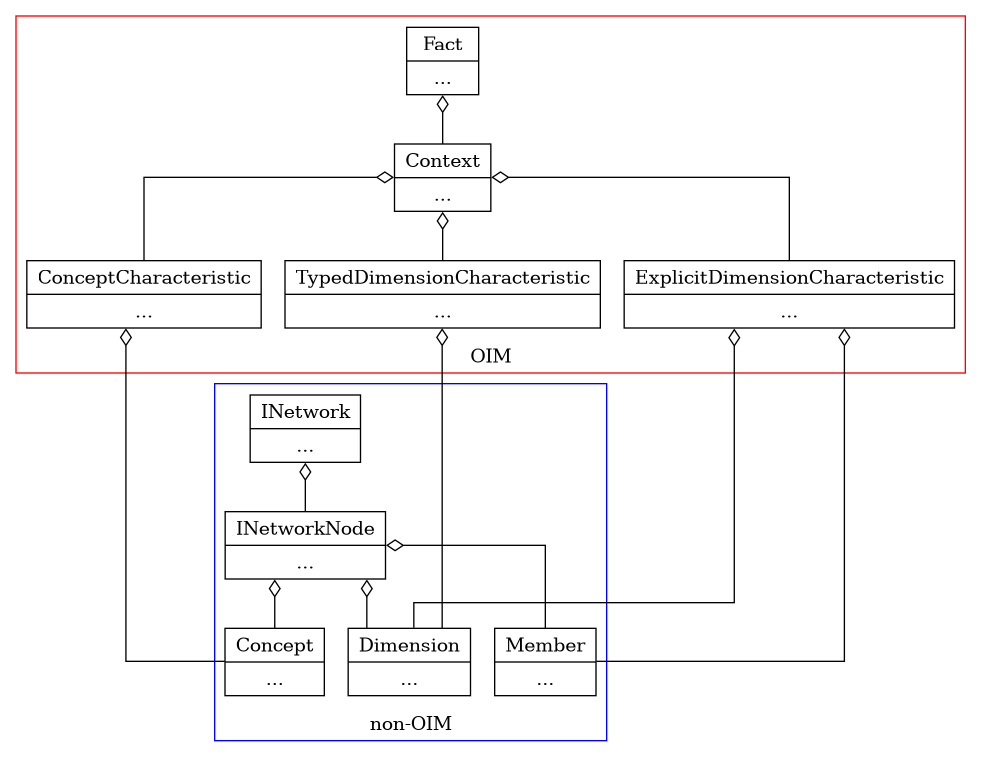
\includegraphics[width=0.8\textwidth]{images/brel_combine_api.png}
    \caption{The Interaction Between Characteristics and Report Elements}
    \label{fig:brel_combine_api}
\end{figure}

% Where the OIM uses the characteristics to describe facts, networks use the report elements inside the characteristics.
% Of course, the class \texttt{Concept} for example could have just implemented both the \texttt{IReportElement} and the \texttt{ICharacteristic} interface.
% However, concepts in facts and concepts in networks are used in different contexts, and they should not be used interchangeably.
% Therefore, Brel uses two different classes for the two different use cases.
In this setup, while the OIM utilizes characteristics to describe facts, networks employ the report elements within these characteristics. 
For instance, the \texttt{Concept} class could have implemented both the \texttt{IReportElement} and \texttt{ICharacteristic} interfaces. 
However, given that concepts in facts and networks serve different purposes, they should not be interchangeable. 
Consequently, Brel employs different classes for the two distinct use cases.

% However, Brel's API took a detour from the OIM when it introduced report elements.
% % Where the Brel API differs from the OIM so far is in its introduction of report elements.
% Yes, the OIM introduces concepts, dimensions and members, but it does not categorize them under a common umbrella term
% \footnote{The OIM would technically group concepts and members under the term "dimension", 
% but it overloads the term "dimension" so many times that it is not clear what it refers to in any given context.
% This grouping is also different from report elements semantics-wise.}.
% In the OIM, these three terms describe three completely unrelated things, and they are unrelated if one only considers the OIM.
% % Brel simply takes the liberty of grouping them under the term "report element".
% % However, the Brel API also aims to cover the parts of XBRL that are not yet covered by the OIM.
% % The non-OIM parts of XBRL are networks, components and resources.
% % Networks require elements like concepts, dimensions and members to be treated in a homogeneous way.
% % The exact reasoning behind this will be explained in the second half of this chapter.
% Brel simply takes the liberty of grouping them under the term "report element".
% It then renames the report elements by introducing the "characteristic" suffix.
% So instead of "concept", Brel uses "concept characteristic", which is a different class in the Brel API.
% % The way Brel bridges the gap between the OIM and the non-OIM parts of XBRL is by introducing characteristics and report elements.

% Characteristics are used for facts, while report elements are used for networks.
% This is the reason why Brel uses \texttt{ConceptCharacteristic} instead of \texttt{Concept} when talking about the concept characteristic of a fact.
% Sure, a \texttt{ConceptCharacteristic} is in essence a wrapper around a \texttt{Concept}, 
% but the two classes are used in different contexts.

% This concludes the chapter on the Brel API.
% It covered both the OIM and the non-OIM parts of XBRL.
% It also explained how the two parts can be combined into a single API, in turn answering both research questions \ref{RQ1} and \ref{RQ2}.
% With both the API and the underlying XBRL standard covered, the next chapter will introduce the implementation of the Brel API.
% This marks the end of the chapter on the Brel API.

\section{API Summary}

This concludes the chapter on the Brel API.
It addressed both the OIM and non-OIM elements of XBRL.
Additionally, it detailed how these components are integrated into a singular API, thereby addressing research questions \ref{RQ1} and \ref{RQ2}.
Following this comprehensive coverage of the API and the foundational XBRL standard, the subsequent chapter will focus on the implementation of the Brel API.